\begin{frame}{Diamond Types}

	\begin{itemize}
		\itemfill
		\item diamonds artificially grown with chemical vapour deposition (CVD)
		\item investigation of two different diamond types:
	\end{itemize}
	
	\begin{figure}[h] 
		\centering
		\begin{subfigure}{0.45\textwidth}  
			\centering
			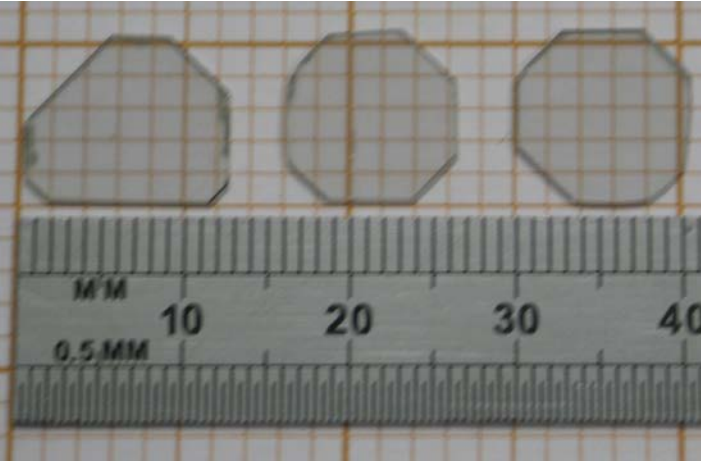
\includegraphics[height=0.4\textheight]{scDia}
			\caption{single-crystalline CVD}
		\end{subfigure}
		\begin{subfigure}{0.45\textwidth} 
			\centering
			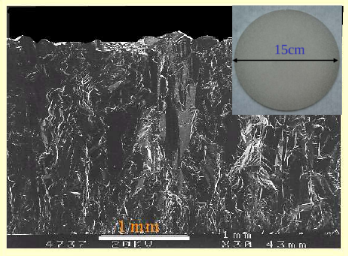
\includegraphics[height=0.4\textheight]{pCVD1}
			\caption{poly-crystalline CVD (courtesy of E6)} 	
		\end{subfigure} 
	\end{figure}\vspace*{-5pt}
	
	\hspace*{10pt}
	\begin{minipage}{5.5cm}
		\begin{itemize}
% 			\item grown on existing diamond crystal
			\item only small sizes (\SI{\sim.25}{cm^2})
% 			\item larger signals than pCVD ($5:3$)
%  			\item full charge collection
		\end{itemize}
	\end{minipage}
	\hspace*{2pt}
	\begin{minipage}{5.5cm}
		\begin{itemize}
% 			\item grown on Si substrate with diamond powder
			\item large wafers (\SIrange{5}{6}{''} \diameter)
% 			\item non-uniformities and grains
% 			\item collection distance up to \SI{500}{\micro\meter}
		\end{itemize}
	\end{minipage}
	
	\begin{itemize}
		\item pCVD signals smaller than scCVD (1:2) in planar configuration
	\end{itemize}

	
\end{frame}
